\documentclass[../slides]{subfiles}

\begin{document}
    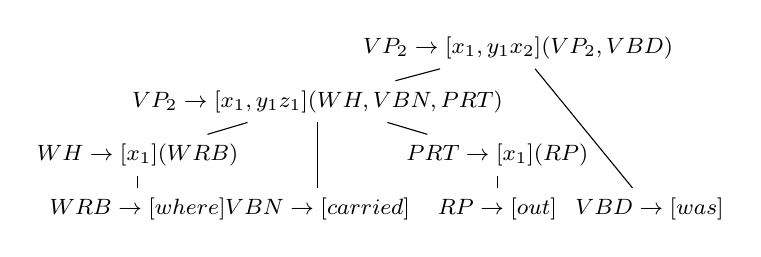
\begin{tikzpicture}[
%        edge from parent path={(\tikzparentnode.south) -- ++(0,-.5ex) -| (\tikzchildnode.north)},
%        every path/.style={line width=.2ex},
        level distance=4.5ex,
        %      node distance=3ex,
%        anchor=center,
        every node/.style={font=\footnotesize}
        ]
            \node (vp1) {\(VP_2 \to [x_1, y_1 x_2] (VP_2, VBD)\)}
                [sibling distance=6.5em]
                child { node[xshift=-4em] (vp2) {\(VP_2 \to [x_1, y_1 z_1] (WH, VBN, PRT)\)}
                    child { node (wh) {\(WH \to [x_1] (WRB)\)} child {
                            node (term0) {\(WRB \to [\text{where}]\)}}}
                    child {
                        node[yshift=-4.5ex](term4) {\(VBN \to [\text{carried}]\)}}
                    child { node (prt) {\(PRT \to [x_1](RP)\)} child {
                            node (term5) {\(RP \to [\text{out}]\)}}}}
                child {
                    node[yshift=-9ex, xshift=1.5em] (term3) {\(VBD \to [\text{was}]\)}};


%        \node (sbar) {\(SBAR \to [x_1](S)\)}
%        child { node (s) {\(S \to [x_1 y_1 x_2] (VP_2, NP)\)}
%            [sibling distance=7em]
%            child { node (vp1) {\(VP_2 \to [x_1, y_1 x_2] (VP_2, VBD)\)}
%                [sibling distance=6.5em]
%                child { node[xshift=-4em] (vp2) {\(VP_2 \to [x_1, y_1 z_1] (WH, VBN, PRT)\)}
%                    child { node (wh) {\(WH \to [x_1] (WRB)\)} child {
%                            node (term0) {\(WRB \to [\text{where}]\)}}}
%                    child {
%                        node[yshift=-4.5ex](term4) {\(VBN \to [\text{carried}]\)}}
%                    child { node (prt) {\(PRT \to [x_1](RP)\)} child {
%                            node (term5) {\(RP \to [\text{out}]\)}}}}
%                child {
%                    node[yshift=-9ex, xshift=1.5em] (term3) {\(VBD \to [\text{was}]\)}}}
%            child { node[yshift=-9ex, xshift=10em] (np) {\(NP \to [x_1 y_1](PT, NN)\)}
%                child { node (term1) {\(PT \to [the]\)} }
%                child {
%                    node (term2) {\(NN \to [\text{survey}]\)}}}};
    \end{tikzpicture}
\end{document}